\documentclass[de]{./../../common/SurferDesc}%%%%%%%%%%%%%%%%%%%%%%%%%%%%%%%%%%%%%%%%%%%%%%%%%%%%%%%%%%%%%%%%%%%%%%%
%
% The document starts here:
%
\begin{document}
\footnotesize
% Weltrekordfl�chen

%%% 1.Tafel

%%%%%%%%%%%%%%%%%%%%%%%%%%%%%


%%%%%%%%%%%%%%%%%%%%%


\begin{surferPage}
  \begin{surferTitle}Die Kummer-Quartik\end{surferTitle}  \\
  Eduard Kummer war 1875 der erste, der explizit die Frage nach der maximalen Anzahl, genannt $\mu(d)$, von Singularit�ten auf einer Fl�che vom Grad d formulierte, und zwar f�r Fl�chen vom Grad 4, d. h. {\it  Quartiken}.\\
Er zeigte, dass $\mu(4) = 16$ ist und untersuchte in der Folgezeit Fl�chen mit dieser Eigenschaft im Detail. Eine besonders sch�ne Familie solcher Fl�chen ist gegeben durch:
\[
\bigl(x^2+y^2+z^2-\mu^2\bigr)^2-\lambda y_0 y_1 y_2 y_3,
\]
wobei $\mu$ ein frei w�hlbarer Parameter ist  und $\lambda$ von $\mu$ abh�ngt. Die $y_i$ sind, damit die Fl�che symmetrisch ist, als die Seiten eines regelm��igen Tetraeders  {\small
    $y_0=1-z-\sqrt{2}x$, \  
    $y_1=1-z+\sqrt{2}x$, \ 
    $y_2=1+z+\sqrt{2}y$, \ 
    $y_3=1+z-\sqrt{2}y$} gew�hlt. \\
Nicht alle Mitglieder dieser Familie haben genau 16 reelle Singularit�ten, die meisten aber schon. 
\newline

 \begin{center}
      \vspace{-0.2cm}
      \begin{tabular}{@{}c@{\ }c@{\ }c@{\ }c@{}}
        \begin{tabular}{@{}c@{}}
          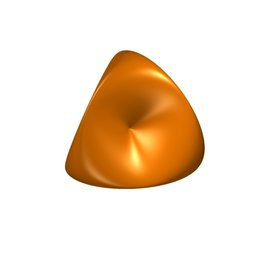
\includegraphics[width=1.35cm]{./../../common/images/kummer_0}
        \end{tabular}
        &
        \begin{tabular}{@{}c@{}}
          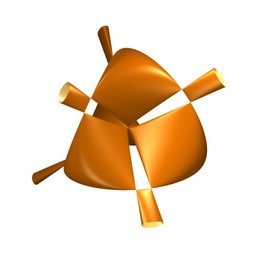
\includegraphics[width=1.35cm]{./../../common/images/kummer_1}
        \end{tabular}
        &
        \begin{tabular}{@{}c@{}}
          
\includegraphics[width=1.35cm]{./../../common/images/kummer_2}
        \end{tabular}
        &
        \begin{tabular}{@{}c@{}}
          
\includegraphics[width=1.35cm]{./../../common/images/kummer_3}
        \end{tabular}
      \end{tabular}
    \end{center}
      \vspace{-0.2cm}  
  F\"ur spezielle Werte der Parameter k\"onnen mehrere Singularit\"aten aufeinander fallen.

  \begin{surferText}
     \end{surferText}
\end{surferPage}
%%%%%%%%%%%%%%%%%%%%%%%%%%%%%


\end{document}
%
% end of the document.
%
%%%%%%%%%%%%%%%%%%%%%%%%%%%%%%%%%%%%%%%%%%%%%%%%%%%%%%%%%%%%%%%%%%%%%%%
